% questions.tex —— 2002 年·春季京蒙皖卷·理科 · 题目内容片段（无答案）
% 由 tools/generate_projects.py 依来源总账自 2002/2002_数学真题_春季京蒙皖理_试题.md 生成，勿手改（改源 MD 后重跑）


\gkpart{数学}

\begin{gktip}
\textbf{来源说明}：本题面依据固定源 PDF 两页题面逐题转录，原卷印刷页码 95–96。固定源不附答案，答案和解析均由本库独立复算。

\textbf{图形说明}：第 15、19 题的原卷图形关系重绘为 TikZ/PGFPlots 矢量图。图形标记所指的 PNG 不随仓库保存。
\end{gktip}

\gkpart{一、选择题}

\begin{question}
\gkti{1}不等式组

\nopagebreak[4]
\[
\begin{cases}
x^2-1<0,\\
x^2-3x<0
\end{cases}
\]

的解集为\mbox{（　　）}

（A）$\{x\mid -1<x<1\}$　　（B）$\{x\mid 0<x<3\}$

（C）$\{x\mid 0<x<1\}$　　（D）$\{x\mid -1<x<3\}$

\end{question}
\begin{question}
\gkti{2}已知三条直线 $m\text{、}n\text{、}l$，三个平面 $\alpha\text{、}\beta\text{、}\gamma$，下列四个命题中，正确的是\mbox{（　　）}

（A）$\begin{cases}\alpha\perp\gamma,\\ \beta\perp\gamma\end{cases}\Rightarrow\alpha\parallel\beta$

（B）$\begin{cases}m\parallel\beta,\\ l\perp m\end{cases}\Rightarrow l\perp\beta$

（C）$\begin{cases}m\parallel\gamma,\\ n\parallel\gamma\end{cases}\Rightarrow m\parallel n$

（D）$\begin{cases}m\perp\gamma,\\ n\perp\gamma\end{cases}\Rightarrow m\parallel n$

\end{question}
\begin{question}
\gkti{3}已知椭圆的焦点是 $F_1\text{、}F_2$，$P$ 是椭圆上的一个动点。如果延长 $F_1P$ 到 $Q$，使得 $|PQ|=|PF_2|$，那么动点 $Q$ 的轨迹是\mbox{（　　）}

（A）圆　　（B）椭圆　　（C）双曲线的一支　　（D）抛物线

\end{question}
\begin{question}
\gkti{4}如果 $\theta\in\left(\dfrac\pi2,\pi\right)$，那么复数

\nopagebreak[4]
\[
(1+i)(\cos\theta+i\sin\theta)
\]

的辐角的主值是\mbox{（　　）}

（A）$\theta+\dfrac{9\pi}{4}$　　（B）$\theta+\dfrac\pi4$　　（C）$\theta-\dfrac\pi4$　　（D）$\theta+\dfrac{7\pi}{4}$

\end{question}
\begin{question}
\gkti{5}若角 $\alpha$ 满足 $\sin2\alpha<0$，$\cos\alpha-\sin\alpha<0$，则 $\alpha$ 在\mbox{（　　）}

（A）第一象限　　（B）第二象限　　（C）第三象限　　（D）第四象限

\end{question}
\begin{question}
\gkti{6}从 6 名志愿者中选出 4 人分别从事翻译、导游、导购、保洁四项不同工作。若其中甲、乙两名志愿者都不能从事翻译工作，则选派方案共有\mbox{（　　）}

（A）280 种　　（B）240 种　　（C）180 种　　（D）96 种

\end{question}
\begin{question}
\gkti{7}在 $\triangle ABC$ 中，$AB=2$，$BC=1.5$，$\angle ABC=120^\circ$。若使三角形绕直线 $BC$ 旋转一周，则所形成的几何体的体积是\mbox{（　　）}

（A）$\dfrac32\pi$　　（B）$\dfrac52\pi$　　（C）$\dfrac72\pi$　　（D）$\dfrac92\pi$

\end{question}
\begin{question}
\gkti{8}圆 $2x^2+2y^2=1$ 与直线

\nopagebreak[4]
\[
x\sin\theta+y-1=0
\qquad\left(\theta\in\mathbb R,\ \theta\ne\frac\pi2+k\pi,\ k\in\mathbb Z\right)
\]

的位置关系是\mbox{（　　）}

（A）相交　　（B）相切　　（C）相离或相切　　（D）不能确定

\end{question}
\begin{question}
\gkti{9}在极坐标系中，如果一个圆的方程

\nopagebreak[4]
\[
\rho=4\cos\theta+6\sin\theta,
\]

那么过圆心且与极轴平行的直线方程是\mbox{（　　）}

（A）$\rho\sin\theta=3$　　（B）$\rho\sin\theta=-3$　　（C）$\rho\cos\theta=2$　　（D）$\rho\cos\theta=-2$

\end{question}
\begin{question}
\gkti{10}对于二项式

\nopagebreak[4]
\[
\left(\frac1x+x^3\right)^n\qquad(n\in\mathbb N^*),
\]

四位同学作出了四种判断：

① 存在 $n\in\mathbb N^*$，展开式中有常数项；

② 对任意 $n\in\mathbb N^*$，展开式中没有常数项；

③ 对任意 $n\in\mathbb N^*$，展开式中没有 $x$ 的一次项；

④ 存在 $n\in\mathbb N^*$，展开式中有 $x$ 的一次项。

上述判断中正确的是\mbox{（　　）}

（A）①与③　　（B）②与③　　（C）①与④　　（D）②与④

\end{question}
\begin{question}
\gkti{11}若一个等差数列前 3 项的和为 34，最后 3 项的和为 146，且所有项的和为 390，则这个数列有\mbox{（　　）}

（A）13 项　　（B）12 项　　（C）11 项　　（D）10 项

\end{question}
\begin{question}
\gkti{12}用一张钢板制作一个容积为 $4\text{ m}^3$ 的无盖长方体水箱。可用的长方形钢板有四种不同的规格（长$\times$宽的尺寸如各选项所示，单位均为 m），若既要够用，又要所剩最少，则应选钢板的规格是\mbox{（　　）}

（A）$2\times5$　　（B）$2\times5.5$　　（C）$2\times6.1$　　（D）$3\times5$

\end{question}
\gkpart{二、填空题}

\begin{question}
\gkti{13}若双曲线

\nopagebreak[4]
\[
\frac{x^2}{4}-\frac{y^2}{m}=1
\]

的渐近线方程为 $y=\pm\dfrac{\sqrt3}{2}x$，则双曲线的焦点坐标是\gkblank{}。

\end{question}
\begin{question}
\gkti{14}如果 $\cos\theta=-\dfrac{12}{13}$，$\theta\in\left(\pi,\dfrac{3\pi}{2}\right)$，那么

\nopagebreak[4]
\[
\cos\left(\theta+\frac{3\pi}{4}\right)
\]

的值等于\gkblank{}。

\Needspace{0.4\textheight}
\end{question}
\begin{question}
\gkti{15}正方形 $ABCD$ 的边长是 2，$E\text{、}F$ 分别是 $AB$ 和 $CD$ 的中点，将正方形沿 $EF$ 折成直二面角（如图所示）。$M$ 为矩形 $AEFD$ 内一点，如果 $\angle MBE=\angle MBC$，$MB$ 和平面 $BCF$ 所成角的正切值为 $\dfrac12$，那么点 $M$ 到直线 $EF$ 的距离为\gkblank{}。
\nopagebreak[4]
\begin{center}% 2002 年春季京蒙皖理卷第 15 题：正方形折叠成直二面角
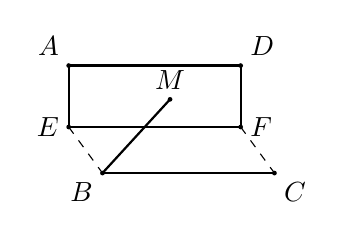
\begin{tikzpicture}[scale=0.78]
  \coordinate (A) at (0,2);
  \coordinate (D) at (2.8,2);
  \coordinate (E) at (0,1);
  \coordinate (F) at (2.8,1);
  \coordinate (B) at (0.55,0.25);
  \coordinate (C) at (3.35,0.25);
  \coordinate (M) at (1.65,1.45);

  \draw[thick] (A)--(D)--(F)--(E)--cycle;
  \draw[thick] (E)--(F);
  \draw[thick] (B)--(C);
  \draw[dashed] (E)--(B) (F)--(C);
  \draw[thick] (B)--(M);

  \fill (A) circle (1.1pt) node[above left] {$A$};
  \fill (D) circle (1.1pt) node[above right] {$D$};
  \fill (E) circle (1.1pt) node[left] {$E$};
  \fill (F) circle (1.1pt) node[right] {$F$};
  \fill (B) circle (1.1pt) node[below left] {$B$};
  \fill (C) circle (1.1pt) node[below right] {$C$};
  \fill (M) circle (1.1pt) node[above] {$M$};
\end{tikzpicture}
\end{center}
\nopagebreak[4]
\end{question}
\begin{question}
\gkti{16}对于任意两个复数 $z_1=x_1+y_1i$、$z_2=x_2+y_2i$（$x_1\text{、}y_1\text{、}x_2\text{、}y_2$ 为实数），定义运算 $\odot$ 为

\nopagebreak[4]
\[
z_1\odot z_2=x_1x_2+y_1y_2.
\]

设非零复数 $w_1\text{、}w_2$ 在复平面内对应的点分别为 $P_1\text{、}P_2$，点 $O$ 为坐标原点。如果 $w_1\odot w_2=0$，那么在 $\triangle P_1OP_2$ 中，$\angle P_1OP_2$ 的大小为\gkblank{}。

\end{question}
\gkpart{三、解答题}

\begin{question}
\gkti{17}在 $\triangle ABC$ 中，已知 $A\text{、}B\text{、}C$ 成等差数列，求

\nopagebreak[4]
\[
\tan\frac A2+\tan\frac C2+\sqrt3\tan\frac A2\tan\frac C2
\]

的值。

\end{question}
\begin{question}
\gkti{18}已知函数 $f(x)$ 是偶函数，而且在 $(0,+\infty)$ 上是增函数，判断 $f(x)$ 在 $(-\infty,0)$ 上是增函数还是减函数，并证明你的判断。

\Needspace{0.4\textheight}
\end{question}
\begin{question}
\gkti{19}在三棱锥 $S-ABC$ 中，如图，$\angle SAB=\angle SAC=\angle ACB=90^\circ$，$AC=2$，$BC=\sqrt{13}$，$SB=\sqrt{29}$。
\nopagebreak[4]
\begin{center}% 2002 年春季京蒙皖理卷第 19 题：三棱锥空间图形
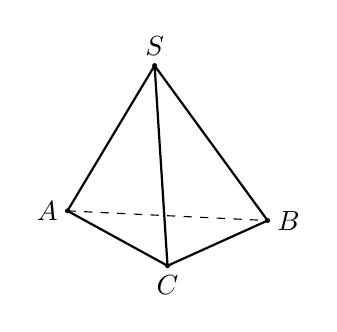
\begin{tikzpicture}[>=stealth, scale=0.82]
  \coordinate (A) at (0,0);
  \coordinate (C) at (1.55,-0.85);
  \coordinate (B) at (3.1,-0.15);
  \coordinate (S) at (1.35,2.25);

  \draw[thick] (A)--(C)--(B);
  \draw[dashed] (A)--(B);
  \draw[thick] (S)--(A) (S)--(B) (S)--(C);

  \fill (A) circle (1.1pt) node[left] {$A$};
  \fill (B) circle (1.1pt) node[right] {$B$};
  \fill (C) circle (1.1pt) node[below] {$C$};
  \fill (S) circle (1.1pt) node[above] {$S$};
\end{tikzpicture}
\end{center}
\nopagebreak[4]
（1） 证明：$SC\perp BC$；

（2） 求侧面 $SBC$ 与底面 $ABC$ 所成的二面角大小；

（3） 求异面直线 $SC$ 与 $AB$ 所成的角的大小（用反三角函数表示）。

\end{question}
\begin{question}
\gkti{20}假设 A 型进口车关税税率在 2001 年是 100\%，在 2006 年是 25\%，2001 年 A 型进口车每辆价格为 64 万元（其中含 32 万元关税税款）。

（1） 已知与 A 型车性能相近的 B 型国产车，2001 年每辆价格为 46 万元。若 A 型车的价格只受关税降低的影响，为了保证 2006 年 B 型车的价格不高于 A 型车价格的 90\%，B 型车价格要逐年降低，问平均每年至少下降多少万元？

（2） 某人在 2001 年将 33 万元存入银行，假设银行扣利息税后的年利率为 1.8\%（5 年内不变），且每年按复利计算（上一年的利息计入第二年的本金），那么五年到期时这笔钱连本带息是否一定够买按（1）中所述降价后的 B 型车一辆？

\end{question}
\begin{question}
\gkti{21}已知点的序列 $A_n(x_n,0)$，$n\in\mathbb N$，其中 $x_1=0$，$x_2=a$（$a<0$），$A_3$ 是线段 $A_1A_2$ 的中点，$A_4$ 是线段 $A_2A_3$ 的中点，$\cdots$，$A_n$ 是线段 $A_{n-2}A_{n-1}$ 的中点，$\cdots$。

（1） 写出 $x_n$ 与 $x_{n-1}\text{、}x_{n-2}$ 之间的关系式（$n\ge3$）；

（2） 设 $a_n=x_{n+1}-x_n$，计算 $a_1\text{、}a_2\text{、}a_3$，由此推测数列 $\{a_n\}$ 的通项公式，并加以证明；

（3） 求 $\displaystyle\lim_{n\to\infty}x_n$。

\end{question}
\begin{question}
\gkti{22}已知某椭圆的焦点是 $F_1(-4,0)$、$F_2(4,0)$，过点 $F_2$ 并垂直于 $x$ 轴的直线与椭圆的一个交点为 $B$，且 $|F_1B|+|F_2B|=10$。椭圆上不同的两点 $A(x_1,y_1)$、$C(x_2,y_2)$ 满足条件：$|F_2A|\text{、}|F_2B|\text{、}|F_2C|$ 成等差数列。

（1） 求该椭圆的方程；

（2） 求弦 $AC$ 中点的横坐标；

（3） 设弦 $AC$ 的垂直平分线的方程为 $y=kx+m$，求 $m$ 的取值范围。

\end{question}